\documentclass[../main.tex]{subfiles}
\begin{document}

In der Bewertung der Ergebnisse muss nun auf Grundlage der erzeugten Datei die Entscheidung getroffen, ob der Code compliant oder nicht ist.
Bisher wurde diese Entscheidung nicht eindeutig nach den Richtlinien getroffen.
Stattdessen wurde sie weitgehend von Piper übernommen.
Problem ist, dass dieser Prozess mit Piper nicht durchsichtig ist und keine Verantwortungen abgeklärt sind.
Es bedarf einer Lösung, die flexibel, falls sich die Anforderungen an Code und damit die Richtlinien ändern, und nachvollziehbar, sodass immer klar ist auf welcher Grundlage die Entscheidung getroffen wurde, ist.

Von der SAP Abteilung Hyperspace werden seit neusten Richtlinien in einem \gls{glos:PolicyAsCode} Format bereitgestellt.
Diese Richtlinien sind in der sogenannten Rego Programmiersprache formuliert, die mit dem \gls{OPA} angewandt werden können.
Dieser \gls{OPA} wird von Hyperspace genutzt.

\begin{figure}[ht]
    \centering
    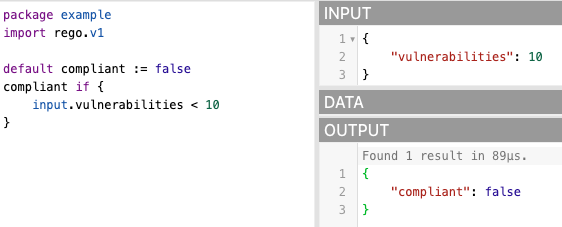
\includegraphics[scale=0.65]{bilder/regoexample.png}
    \caption{Beispiel Rego Script mit Ein- und Ausgabe (selbst geschrieben)}
    \label{fig:regoexample}
\end{figure}

Das in Abbildung \ref{fig:regoexample} zu sehende Script ist immer eindeutig, transparent und schnell anzupassen.
Die verwendete Rego Programmiersprache ist außerdem dafür optimiert Richtlinien anzuwenden.
Damit is der \gls{OPA} mit Rego für die genannten Anforderungen geeignet.
\cite{Rego}

Genutzt werden können diese Richtlinien von Hyperspace in zwei Schritten.

Als erstes wird die Ergebnisdatei des Scans auf einen Server von Hyperspace hochgeladen.
In dem Upload ist noch eine sogenannter Policy Key (Deutsch: Richtlinien Schlüssel) enthalten, der eindeutig zuordnet, welche Richtlinie für das Ergebnis genutzt werden soll.
So können dann die Ergebnisse des Scans bei Hyperspace mit Hilfe von \gls{OPA} ausgewertet werden.

Im zweiten Schritt müssen die Auswertungsergebnisse dann innerhalb der \gls{glos:pipeline} nutzbar gemacht werden.
Dafür wird eine Anfrage an den Hyperspace Server geschickt, der eine Datei mit der Auswertung zurückgibt.
Diese Datei enthält im \gls{glos:JSON} Format die Information, ob der gescannte Code der Richtlinie mit gegebenen Policy Key entspricht oder nicht.

Da die Evaluation auf dem Hyperspace Server asynchron läuft und nicht klar ist, wann die Auswertung zur Verfügung steht, wird ein Fallback-Mechanismus implementiert, der diese zweite Anfrage in größer werdenden Zeitabständen bis zu fünf Mal wiederholt.
Wenn es nach dem fünften Versuch kein Ergebnis gibt, bricht die Bewertung ab und das Check Gesamtergebnis wird als unbekannt gesetzt.

Damit für den Endbenutzer dieser Entscheidungsfindungsprozess nachvollziehbar bleibt, werden mit einer dritten Anfrage an den Hyperspace Server Details zu der Auswertung abgerufen.
Diese Details werden dem Benutzer zusätzlich zu dem eigentlichen Auswertungsergebnis - compliant oder nicht - angezeigt.
Sie enthalten Informationen wie den Namen der Richtlinie, eine Kurzbeschreibung, die URL zu der genutzten Richtlinie im \gls{glos:PolicyAsCode} Format sowie noch einiges mehr.


\end{document}